\chapter{Approximating $\sqrt{n}$ with the Babylonian Method}

\setcounter{problem}{1}
\section{Motivation}

\begin{fullwidth}

This lab is really a fancy way to learn about looping in Python and how to quickly prototype something in Excel (if warranted). It also gets you used to encoding mathematical expressions and recurrence relations in Python.
 
\section{Discussion}

To approximate square root, $\sqrt{n}$, the idea is to pick an initial estimate, $x_0$, and then iterate with better and better estimates, $x_{i}$, using the recurrence relation:

\[
x_{i+1} = \frac{1}{2} (x_i + \frac{n}{x_i})
\]

To see how this works, jump into Excel (yes, a spreadsheet) and crank through a few iterations by defining cells with $n$ and your initial estimate $x_0$, which can be anything you want. (It's sometimes easier to play around without having to deal with a programming language.) Then you need to define a cell that computes the above better approximation using $x_i$ as the cell above it. I hardcoded the names in column A and the first two rows of column B. Cell B3 should be a formula that computes B4 based upon B3. Then you can extend the formula down and watch it converge on the final (correct) value for $\sqrt{125348}$. My spreadsheet looks like this:

~\\
\scalebox{.25}{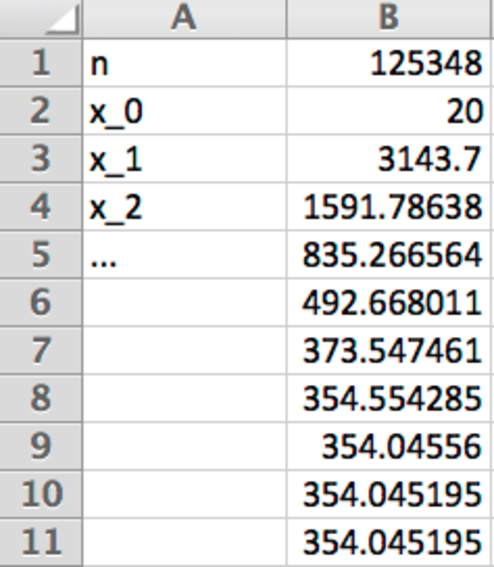
\includegraphics{figures/sqrt-excel.pdf}}
~\\

Try out any nonnegative number and you'll see that it still converges, though at different rates.

There's a great deal on the web you can read to learn more about why this process works but it relies on the average (midpoint) of $x$ and $n/x$ getting us closer to $\sqrt{n}$.  It can be shown that if $x$ is above $\sqrt{n}$ then $n/x$ is below $\sqrt{n}$ and the reverse is true if $x$ is below the root.  The iteration converges and does so quickly. Informally, as shown in Wikipedia, we can represent the true square root by adding an error term to our estimate:

\[
\sqrt{n} = x + \epsilon
\]

or,

\[
n = (x + \epsilon)^2
\]

Expanding, we get:

\[
n = x^2 + 2x\epsilon + \epsilon^2
\]

Solving for $\epsilon$:

\[
n - x^2 = \epsilon (2x + \epsilon)
\]

\[
\epsilon = \frac{n - x^2}{2x + \epsilon}
\]

Because $\epsilon$ is much smaller than $x$, we can drop it from the denominator leaving us with an estimate of epsilon:

\[
\epsilon = \frac{n - x^2}{2x}
\]

Then we can plug it back into $x + \epsilon$ and get:

\[
x := x + \epsilon = x + \frac{n - x^2}{2x} = \frac{2x^2}{2x} + \frac{n - x^2}{2x} = \frac{1}{2}\frac{x^2 + n}{x} = \frac{1}{2}(x + \frac{n}{x})
\]

Which gets its back to the Babylonian formula. Since we dropped an $\epsilon$ term, this formula for $x$ is inexact but it gets us closer to $\sqrt{n}$.

\cut{
To play first use Excel: 
=0.5*(B2+\$B\$1/B2)
}

Now that you understand how this estimate works, your goal is to implement a simple Python method called sqrt() that uses the Babylonian method to approximate the square root. Here is a starter kit for you. Please call the file {\tt sqrt.py}.

\begin{pyverbatim}
import math

# Stop iterating when the new approximation is within
# PRECISION of the old value.
PRECISION = 0.000001

# compute square root of n
def sqrt(n):
    x_0 = 1.0 # pick any old value
    ... fill this in ...

def check(n):
    delta = math.sqrt(n) - sqrt(n)
    if math.abs(delta) > PRECISION:
        raise BaseException("Inaccurate sqrt(%f)=%f; estimate is %f" %
            (n, math.sqrt(n), sqrt(n)))

# check a range of values
check(125348)
check(100)
check(1)
check(0)
\end{pyverbatim}

\section{Deliverables}

Please submit:

\begin{itemize}
\item a PDF showing a snapshot of your spreadsheet
\item the formula you used in B3 {\bf and} B4.
\item your {\tt sqrt.py} Python file
\end{itemize}

{\em You may not use math.sqrt() for implementing your function, but you may use it for testing the results.  Obviously.}

\end{fullwidth}
